%\begin{figure}[H]
%    \centering
    \scalebox{0.95}{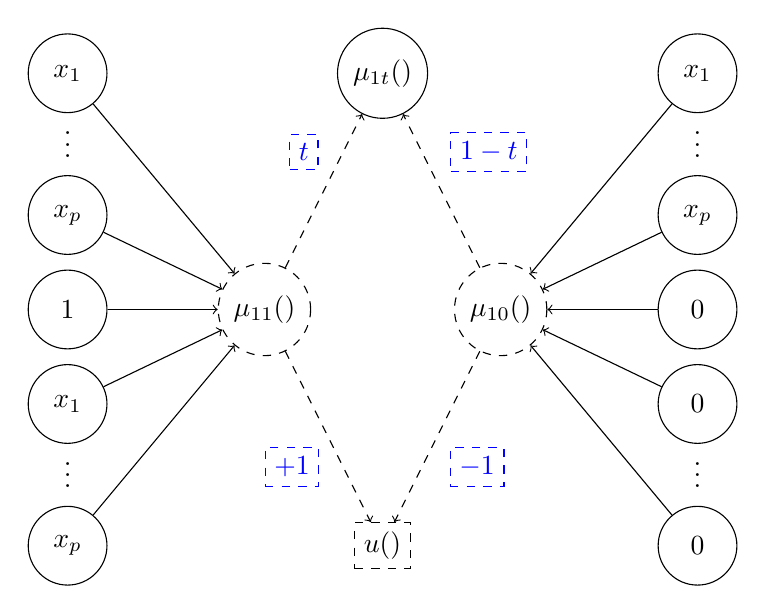
\begin{tikzpicture}
    
    
    \tikzset{dist/.style={path picture= {
    \begin{scope}[x=1pt,y=10pt]
      \draw plot[domain=-6:6] (\x,{1/(1 + exp(-\x))-0.5});
    \end{scope}
    }}}
    \tikzstyle{sigmoid}=[draw,fill=gray!20,circle,minimum size=30pt,inner sep=0pt,dist]
    
    
    % INPUT LAYER
    % T=1
    %\draw[red,thick,dashed] (0,2) circle (3mm);
    \node(x11) at (0,2) [circle,draw, minimum size=1cm] {$x_1$};
    \node at (0,1.2) {$\vdots$};
    %\draw[red,thick,dashed] (0,0) circle (3mm);
    \node(x1p) at (0,0.2) [circle,draw, minimum size=1cm] {$x_p$};
    %\draw[blue,thick,dashed] (0,-1) circle (3mm);
    \node(t1) at (0,-1) [circle,draw, minimum size=1cm] {$1$};
    %\draw[blue,thick,dashed] (0,-2) circle (3mm);
    \node(t1x11) at (0,-2.2) [circle,draw, minimum size=1cm] {$x_1$};
    \node at (0,-3) {$\vdots$};
    %\draw[blue,thick,dashed] (0,-4) circle (3mm);
    \node(t1x1p) at (0,-4) [circle,draw, minimum size=1cm] {$x_p$};
    
    % T=t
    %\draw[red,thick,dashed] (4,-1) circle (3mm);
    %\node(true_t) at (4,-1) {$t$};
    
    % T=0
    %\draw[red,thick,dashed] (8,2) circle (3mm);
    \node(x21) at (8,2) [circle,draw, minimum size=1cm] {$x_1$};
    \node at (8,1.2) {$\vdots$};
    %\draw[red,thick,dashed] (8,0) circle (3mm);
    \node(x2p) at (8,0.2) [circle,draw, minimum size=1cm] {$x_p$};
    %\draw[blue,thick,dashed] (8,-1) circle (3mm);
    \node(t0) at (8,-1) [circle,draw, minimum size=1cm] {$0$};
    %\draw[blue,thick,dashed] (8,-2) circle (3mm);
    \node(t0x21) at (8,-2.2) [circle,draw, minimum size=1cm] {$0$};
    \node at (8,-3) {$\vdots$};
    %\draw[blue,thick,dashed] (8,-4) circle (3mm);
    \node(t0x2p) at (8,-4) [circle,draw, minimum size=1cm] {$0$};
    
    % CONDITIONAL MEANS 
    %\node (p1)[sigmoid] at (2.5, -1) {};
    \node (p1)[] at (2.5, -1) [circle, draw, dashed] {$\mu_{11}(\x)$};
    %\node (p0)[sigmoid] at (5.5, -1) {};
    \node (p0)[] at (5.5, -1) [circle, draw, dashed] {$\mu_{10}(\x)$};
    
    % WEIGHTS
    \draw[->] (x11) -- (p1) ;% node [midway,above]% {$\beta_1$};
    \draw[->] (x1p) -- (p1) ;% node [midway,above] {$\beta_p$};
    \draw[->] (t1) -- (p1) ;% node [midway,above] {$\gamma$};
    \draw[->] (t1x11) -- (p1) ;% node [midway,above] {$\delta_1$};
    \draw[->] (t1x1p) -- (p1) ;% node [midway,above] {$\delta_p$};
    
    
    \draw[->] (x21) -- (p0) ;% node [midway,above] {$\beta_1$};
    \draw[->] (x2p) -- (p0) ;% node [midway,above] {$\beta_p$};
    \draw[->] (t0) -- (p0) ;% node [midway,above] {$\gamma$};
    \draw[->] (t0x21) -- (p0) ;% node [midway,above] {$\delta_1$};
    \draw[->] (t0x2p) -- (p0) ;% node [midway,above] {$\delta_p$};
    
    %OUTPUT
    %\draw[black,thick] (4,-4) circle (5mm);
    \node(uplift) at (4,-4) [rectangle, draw, dashed] {$u(\x)$};
    
    %\draw[black,thick] (4,2) circle (6mm);
    \node(mean) at (4,2) [circle, draw] {$\mu_{1t}(\x)$};
    
    %OUTPUT CONNEXIONS
    %\draw[->, dashed] (true_t) -- (mean);
    \draw[->, dashed] (p1) -- (mean); %node [midway,above] {$t$};
    \node at (3,1) [rectangle, dashed, blue, draw] {$t$};
    \draw[->, dashed] (p0) -- (mean); %node [midway,above] {$(1-t)$};
    \node at (5.35,1) [rectangle, dashed, blue, draw] {$1-t$};
    
    \draw[->, dashed] (p1) -- (uplift); %node [midway,above] {$+1$};
    \node at (2.85,-3) [rectangle, dashed, blue, draw] {$+1$};
    \draw[->, dashed] (p0) -- (uplift); %node [midway,above] {$-1$};
    \node at (5.2,-3) [rectangle, dashed, blue, draw] {$-1$};
    
    \end{tikzpicture}}
%    \caption{SMITE neural network architecture.}
%    \label{fig:nite}
%\end{figure}
